\chapter{Implementação}
	\chapterprecis{Este capítulo contém explicações sobre trechos não triviais dos códigos referentes aos componentes projetados. Além disso contém informações sobre o procedimento de preparação do Raspberry PI para ser integrado ao sistema.}
	
	\section{Código do Arduino}
		O código do Arduino foi elaborado utilizando o diagrama descrito na \autoref{img7}. O código fonte completo está disponibilizado no Github\footnote{\url{https://www.oficinadanet.com.br/post/14791-o-que-github}}, no link \url{https://github.com/felipefonsecabh/ArduinoCode/blob/ArduinoNoNavigation/ArduinoCode.ino}
		
		\subsection{Leitura dos Sensores}
		
		Para a leitura dos sensores foram utilizadas bibliotecas desenvolvidas e mantidas por terceiros. Essas bibliotecas são de código aberto, ou seja, outros usuários podem contribuir para o desenvolvimento e melhoria do código. Geralmente, os projetos das bibliotecas são disponibilizados no GitHub. É importante verificar a versão das bibliotecas utilizadas, pois uma versão pode funcionar de forma diferente da outra.
		
		Para a leitura dos sensores de temperatura foi utilizada a biblioteca Dallas Temperature, mantida por \textcite{miles2016}. A versão utilizada no projeto é a mais atual (versão 3.7.6). A Dallas Temperature possui uma dependência de uma outra biblioteca. Dessa forma, é necessário utilizar também a biblioteca OneWire, atualmente mantida por \textcite{paul2017}. A versão utilizada desta biblioteca também é a mais atual (2.3.3).
		
		Para a leitura da vazão de água quente, foi utilizada a biblioteca Ultrasonic criada por \textcite{filipeflop2011}. Aparentemente, essa biblioteca não está sendo mantida por ninguém. Existem outras bibliotecas para o sensor ultrassônico HC-SR404 disponíveis na internet. O funcionamento do sensor é descrito em \textcite{adilson2011}.
		
		Para a leitura de vazão de água fria não foi utilizada nenhuma biblioteca. O sensor de vazão consiste em um dispositivo que envia pulsos  ao Arduino. Quanto mais pulsos enviados, maior é a vazão. Para a medição da vazão, é feita uma contagem de pulsos em um intervalo de tempo fixo, e posteriormente esse número é inserido em uma fórmula que retorna o valor da vazão. A contagem de pulsos se dá por interrupção.
		
		Como dito na \autoref{sec:met_arduino}, as funções que fazem a leitura dos sensores e convertem os valores para unidade de engenharia foram as mesmas utilizadas por \textcite{luiz2016}. Não faz parte do escopo desse projeto calibrar os sensores novamente.
		
		O código correspondente a leitura dos valores analógicos é mostrado no \autoref*{cod:arduino}. 
		
		%\pagebreak
		
		\begin{listing}[!htb]
			\begin{minted}[bgcolor=bg,breaklines=true,tabsize=2, baselinestretch=1,fontsize=\footnotesize]{cpp}
			void Temperaturas() {
				// call sensors.requestTemperatures() to issue a global temperature 
				// request to all devices on the bus
				sensors.requestTemperatures();
				
				// print the device information
				for (byte i = 0; i <= 4; i++){
					temp[i] = sensors.getTempC(deviceID[i]);
				}
			}
			
			void VazaoAguaFria(){
				currentTime = millis();
				// Every second, calculate litres/hour
				if (currentTime >= (cloopTime + 1000)){
					cloopTime = currentTime; // Updates cloopTime
					// Pulse frequency (Hz) = 7.5Q, Q is flow rate in L/min.
					vazao_fria = (flow_frequency / 7.5); // (Pulse frequency) / 7.5Q = flowrate in L/min
					flow_frequency = 0; // Reset Counter
				}
			}
			
			void VazaoAguaQuente(){
				float vazao1_sf; //descobrir o porque do nome da variavel
				microsec = ultrasonic.timing();
				cmMsec = ultrasonic.convert(microsec, Ultrasonic::CM);
				nivel = 11.46 - cmMsec;
				vazao1_sf = (0.0537)* pow((nivel * 10), 1.4727);
				if (vazao1_sf > 1){
					vazao_quente = 0.75*vazao_quente + 0.25*vazao1_sf;
				}
			}	
			\end{minted}
			\caption{Funções de Leitura dos sensores}
			\label{cod:arduino}
		\end{listing}
	
		\subsection{Comunicação I2C}
			O Arduino disponibiliza na sua instalação padrão, a biblioteca Wire, que permite o Arduino se comunicar via I2C com outros dispositivos. Neste projeto o Arduino atua como slave da comunicação, ou seja, não inicia a comunicação. Portanto, ele responde a algum dispositivo mestre apenas quando solicitado.
			
			Quando o mestre envia um comando de escrita, atua-se uma interrupção, que executa a função onReceive. Quando o mestre envia uma solicitação de dados, atua-se uma outra interrupção, que executa a função onReceive e posteriormente executa a função onRequest. Em suma, a função onReceive é utilizada para interpretar comandos, como por exemplo ligar ou desligar bomba e aquecedor, e a função onRequest é utilizada para enviar para o mestre dados sobre o processo como por exemplo valores de temperaturas e vazões.
			
			As informações referentes ao sistema foram colocados em uma estrutura de dados. São 7 variáveis do tipo float (4 temperaturas, 2 vazões e ainda o valor da velocidade da bomba, e) e 4 informações digitais (estado da bomba e do aquecedor, estado do botão de emergência, estado da chave local/remoto), que foram agrupadas em um byte. A \autoref{fig:i2c_packet} mostra a estrutura de um pacote I2C enviado pelo mestre. Basicamente, o I2C trafega dados em um array de bytes. O primeiro byte é um número que indica o índice de um comando. Esse valor é arbitrário e é definido pelo desenvolvedor que implementa o protocolo. O segundo byte indica a quantidade de bytes dos dados transmitidos. Esse valor é útil para verificar a consistência do pacote recebido. O restante do frame consiste nos dados propriamente ditos.
			
			\begin{figure}[!htb]	
				%\centering
				\captionsetup{justification=centering}
				\begin{center}
					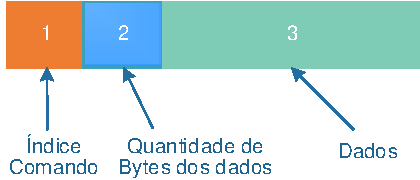
\includegraphics[width=10cm]{i2c_packet}  %pode alterar o tamanho
					\caption[Estrutura de um pacote I2C]{\label{fig:i2c_packet}Estrutura de um pacote I2C}
				\end{center}		
			\end{figure}
			
			Como dito anteriormente, os dados que representam o estado do sistema, não correspondem a um array de bytes. Portanto, foi necessário converter as informações float e digitais para bytes para possibilitar a transmissão do mesmo. No Arduino isso foi feito utilizando a declaração union. Essa técnica permite variáveis de diferentes tipos ocupem uma mesma região de memória, o que possibilita que a estrutura de dados anteriormente criada possua a sua representação em um array de bytes, o que é necessário para transmissão via I2C. O \autoref{cod:dadosi2c} corresponde a implementação feita.
			
			Para correta interpretação dos comandos enviados pelo mestre, foi necessário mapear ações de acordo com o índice de comando criado, ou seja, definir um protocolo básico de comunicação.
			A relação entre o índice de comando e a ação correspondente é mostrada na \autoref{tbl5}. A interpretação e execução dos comandos é feita na função onReceive. Se o comando é uma solicitação de dados, o envio é realizado na função onRequest.
						
			\begin{listing}[!htb]
				\begin{minted}[bgcolor=bg,breaklines=true,tabsize=2, baselinestretch=1,fontsize=\footnotesize]{cpp}
				//estrutura de dados para envio i2c
				typedef struct processData{
					float temp1;
					float temp2;
					float temp3;
					float temp4;
					float hotflow;
					float coldflow;
					float pump_speed;
					byte bstatus;
					byte chksum;
				};
				
				typedef union I2C_Send{ //compartilha a mesma área de memória
					processData data;
					byte I2C_packet[sizeof(processData)];
				};				
				\end{minted}
				\caption{Estrutura de dados do sistema}
				\label{cod:dadosi2c}
			\end{listing}
		
		\begin{table}[!htb]
			\centering
			\caption{Definição das interpretações de comando}
			\label{tbl5}
			\def\arraystretch{1.3}
			\begin{tabular}{c p{11cm}}
				\hline
				\multicolumn{1}{c}{\textbf{Índice Comando}} & \multicolumn{1}{c}{\textbf{Ação}} \\ \hline
				
				6 & Enviar dados do sistema para o mestre \\
				49 & Ligar a bomba \\ %\hline
				50 & Desligar a bomba \\ %\hline  
				51 & Ligar aquecedor \\ %\hline
				52 & Desligar o aquecedor \\ %\hline
				53 & Alterar velocidade da bomba \\ %\hline
				\hline
			\end{tabular}
		\end{table}
		
	\section{Preparação do Raspberry PI}
		\subsection{Instalação do sistema operacional}
			Conforme mencionado na \textcolor{red}{seçãoX}, o Raspberry não possui um HD interno. Portanto, é necessário instalar o sistema operacional em um microUSB, que faz o papel de HD. O Rpi suporta vários sistemas operacionais, sendo que o sistema operacional padrão é o Raspian, uma adaptação de uma distribuição Debian\footnote{\url{https://www.debian.org/intro/about}}. Foi utilizada a versão ``Raspian Stretch With Desktop'', disponível no link \url{https://www.raspberrypi.org/downloads/raspbian/}. Basicamente, deve-se extrair a imagem baixada para o microUSB. Após esse procedimento o Raspberry Pi já pode ser inicializado.
		
		\subsection{Ativação do protocolo I2C}
			O I2C não vem habilitado por padrão no sistema operacional. É necessário entrar nas configurações do Rpi e habilitá-lo. Os passos para realizar esse procedimento estão descritos por \textcite{matt2014}. Para verificar se o i2c está corretamente habilitado, deve-se abrir um terminal e digitar o comando ``sudo i2cdetect -y 1''. O resultado é exibido na \autoref{img9}.
			
			\begin{figure}[!htb]	
				%\centering
				\captionsetup{justification=centering}
				\begin{center}
					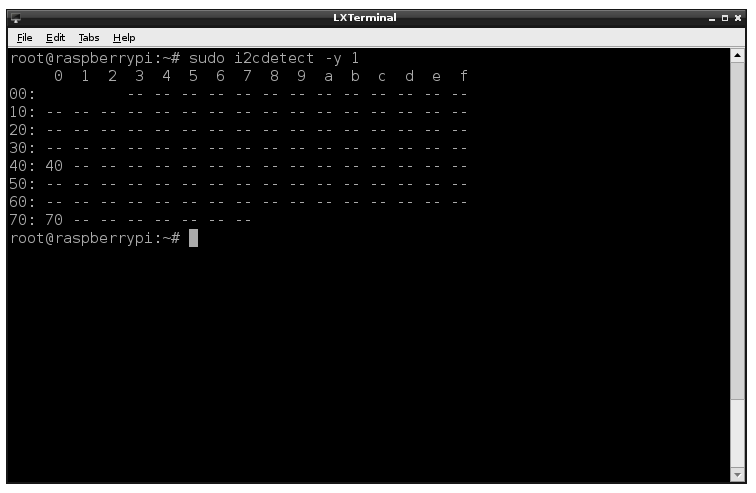
\includegraphics[width=10cm]{img9}  %pode alterar o tamanho
					\caption[I2C habilitado]{\label{img9}I2C habilitado}
				\end{center}		
			\end{figure}
		
		\subsection{Instalação de Pacotes - Python}
			O sistema operacional Raspian já possui duas versões instaladas de Python: 2.7 e 3.4. A primeira, mesmo sendo mais antiga ainda é muito utilizada pela comunidade devido à grande quantidade de pacotes desenvolvidos para essa versão; a segunda, é uma das versões mais novas disponíveis para Python.
			
			Os códigos do Gateway e do WebServer foram desenvolvidos com a versão 3.4. Antes do começo do desenvolvimento é necessário instalar os pacotes necessários para executar o projeto. Os pacotes a serem instalados dependem do propósito e característica do sistema a ser desenvolvido. É muito comum desenvolvedores trabalharem em diferentes projetos, portanto a tarefa de gerenciar os pacotes para cada projeto torna-se trabalhosa. Para isso, o Python disponibiliza a instalação de ambientes virtuais na máquina. Ambientes virtuais são diretórios para armazenar os pacotes necessários para determinados projetos. Assim, é possível isolar os arquivos de cada desenvolvimento, facilitando a mudança de um projeto para o outro \cite{kyle2017}. A utilização de ambientes virutais em Python é uma boa prática de programação e foi utilizada.
			
			Para instalar um ambiente virtual na versão python 3, é necessário utilizar os comandos descritos no \autoref{cod:venv}. Uma vez instalado, é necessário ativar o ambiente virtual. O  \autoref{cod:activate_venv} contém o código para ativá-lo. Após ativado, devem-se instalar os pacotes necessários para o projeto.  Os pacotes e as versões instaladas estão listados na \autoref{tbl6}
			
			\begin{listing}[!htb]
				\begin{minted}[bgcolor=bg,breaklines=true,tabsize=2, baselinestretch=1,fontsize=\footnotesize]{bash}
				#navegar até a pasta onde se deseja instalar o ambiente virtual
				pi@raspberry $ cd pfc_env
				
				#instalar pacote virtual env
				pi@raspberry $ pip install virtualenv
				
				#criar um ambiente virtual chamado env
				pi@raspberry $ virtual env			
				\end{minted}
				\caption{Comandos para criação de um ambiente virtual}
			\label{cod:venv}
			\end{listing}
		
			\begin{listing}[!htb]
				\begin{minted}[bgcolor=bg,breaklines=true,tabsize=2, baselinestretch=1,fontsize=\footnotesize]{bash}
				#ativar o diretório virtual
				pi@raspberry $ source pfc_env/bin/activate
				
				#caso o nome do diretório apareça entre parenteses como abaixo, o diretório foi ativado com sucesso
				(env) pi@raspberry $ 		
				\end{minted}
				\caption{Comandos para criação de um ambiente virtual}
				\label{cod:activate_venv}
			\end{listing}

			
			\begin{table}[!htb]
				\centering
				\caption{Pacotes necessários para o projeto}
				\label{tbl6}
				\def\arraystretch{1.3}
				\begin{tabular}{c c}
					\hline
					\multicolumn{1}{c}{\textbf{Pacote}} & \multicolumn{1}{c}{\textbf{Versão}} \\ \hline
					
					Smbus & v1.9.2 \\
					Django & v1.9.2 \\ %\hline
					Pillow & v1.9.2 \\ %\hline  
					\hline
				\end{tabular}
			\end{table}
		
			\begin{listing}[!htb]
				\begin{minted}[bgcolor=bg,breaklines=true,tabsize=2, baselinestretch=1,fontsize=\footnotesize]{bash}
				#ativar o diretório virtual
				#o comando é pip install NomePacote== Versão. Exemplo:
				(env) pi@raspberry $ pip install Django==1.9.6					
				\end{minted}
				\caption{Comando para a instalação de pacotes Python}
				\label{cod:install}
			\end{listing}
		
			Todos os pacotes, com exceção do Smbus, podem ser instalados através do comando exibido no \autoref{cod:install}. É necessário ativar o ambiente virtual antes de efetuar os comandos. Para a instalação do Smbus, é necessário seguir os passos descritos por \textcite{dipto2015}. 
			
		
		
		\section{Código do Gateway}
			O código fonte completo do gateway está disponibilizado no Github, no link: \url{https://github.com/felipefonsecabh/PFC/blob/PyServeri2c/arduinoserver.py}. Conforme mencionado na \autoref{sec:met_gateway}, o programa consiste em 2 threads que são executadas continuamente, ou seja em loop infinito.
			
			\subsection{Thread 1: Leitura de Dados do Arduino e Escrita no Banco}
				Para implementar a comunicação I2C no Gateway, utiliza-se a biblioteca Smbus. Primeiramente é necessário inicializar a conexão com o Arduino, referenciando o endereço do mesmo. Esse endereço é arbitrário, e deve possuir o mesmo valor no código do Arduino e no Gateway. Foi escolhido o identificador 12 para o endereço do Arduino.
				
				\begin{listing}[!htb]
					\begin{minted}[bgcolor=bg,breaklines=true,tabsize=2, baselinestretch=1,fontsize=\footnotesize]{python}
					#inicialização do i2c
					bus = SMBus(1)
					arduinoAddress = 12				
					\end{minted}
					\caption{Inicialização da comunicação I2C}
					\label{cod:starti2c}
				\end{listing}
				
				A solicitação de dados para o Arduino foi feita através da utilização da função read\_i2c\_block\_data. É necessário passar como parâmetro o endereço do Arduino, o ínidice do comando (foi definido na \autoref{tbl5} que o índice do comando da solicitação de dados era 6), e o número de bytes esperados na resposta. O resultado retorna um array de bytes que deve ser convertido nas variáveis reais de processo. Para realizar essa conversão foi utilizada a função unpack do pacote struct\footnote{\url{https://docs.python.org/2/library/struct.html}}. Um exemplo de pacote recebido do Arduino é mostrada na figuraX.
				
				Portanto, é necessário separar o array de bytes em 7 variáveis float e 2 variáveis do tipo byte. O primeiro byte contém as informações de status digitais, e o segundo byte é apenas um valor para verificação da integridade do pacote. Após a separação em variáveis, os dados foram organizados em um dicionário para facilitar o envio para o banco. \cite{mark2013}.
				
				\begin{listing}[!htb]
					\begin{minted}[bgcolor=bg,breaklines=true,tabsize=2, baselinestretch=1,fontsize=\footnotesize]{python}
					#faz requisicao pelos dados
					block = bus.read_i2c_block_data(arduinoAddress,6,30)
					#conversao do array de bytes em variaveis
					data = unpack('7f2b',bytes(block))
					#inserção dos dados em um dicionário
					bstatus, lastdata, lasttrenddata = parseData(data)			
					\end{minted}
					\caption{Leitura dos dados do Arduino}
					\label{cod:read_arduino}
				\end{listing}
			
				O banco de dados possui 3 tabelas: uma tabela para armazenar o estado mais recente do sistema chamada Registers, outra tabela para armazenar o histórico das variáveis chamada TrendRegisters, e uma tabela para armazenar variáveis de controle (como o modo de operação do sistema por exemplo, e se o armazenamento histórico deve estar habilitado ou não) chamada OperationMode. Para armazenar dados no banco, primeiramente é necessário estabelecer uma conexão com o banco (ver \autoref{cod:connect_bd}). A inserção do dado consiste em acessar a tabela passando como parâmetro o dicionário criado anteriormente; por fim, deve-se executar o método save para concluir a operação (ver \autoref{cod:insert_data}).
				
				\begin{listing}[!htb]
					\begin{minted}[bgcolor=bg,breaklines=true,tabsize=2, baselinestretch=1,fontsize=\footnotesize]{python}
					#estabelece conexão com o banco de dados
					if os.environ.setdefault('DJANGO_SETTINGS_MODULE', 'WebSite.settings'):
						import django
						django.setup()
						from WebSite.operation.models import Registers, OperationMode
						from WebSite.trend.models import TrendRegister
						from django.utils import timezone
					else:
						raise
						sys.exit(1)
					\end{minted}
					\caption{Conexão com o banco de dados}
					\label{cod:connect_bd}
				\end{listing}
			
				\begin{listing}[!htb]
					\begin{minted}[bgcolor=bg,breaklines=true,tabsize=2, baselinestretch=1,fontsize=\footnotesize]{python}
					#envia dado para o banco de dados (lastdata contém últimos dados válidos)
					reg = Registers(**lastdata)
					reg.save()
					
					#envia dado para o banco de dados
					treg = TrendRegister(**lasttrenddata)
					treg.save()
					\end{minted}
					\caption{Código necessário para inserção de dados no banco}
					\label{cod:insert_data}
				\end{listing}
			
				As operações de leitura de banco de dados e escrita no banco são cíclicas, ou seja, executam a cada intervalo de tempo. O intervalo das operações é definido no início do código fonte. O tempo é determinado em milissegundos.
				
				\begin{listing}[!htb]
					\begin{minted}[bgcolor=bg,breaklines=true,tabsize=2, baselinestretch=1,fontsize=\footnotesize]{python}
					#intervalo de execução das operações
					start_time = datetime.now()
					readinterval = 100        #intervalo de leitura do arduino
					sendDBinterval = 600      #intervalo de gravação na tabela Registers
					sendTrendDBinterval = 300 #intervalo de gravação na tabela TrendRegisters
					\end{minted}
					\caption{Intervalo de execução das operações}
					\label{cod:set_interval}
				\end{listing}
			
			\subsection{Thread 2: Recebimento de Comandos do WebServer}
				A segunda thread implementa um servidor TCP que fica escutando na porta 8080. Servidores assíncronos não bloqueiam o processo em que estão sendo executados enquanto aguardam dados de algum cliente. Quando algum dado chega, é chamada uma função callback para processá-lo \cite{pythondoc}. Foi utilizado o pacote asyncore, que é disponibilizado na instalação padrão do Python para implementar o servidor assíncrono. A função callback chamada para interpretar os pacotes é a handle\_read, mostrada no \autoref{cod:handle_read}
				
				O WebServer envia comandos de duas formas. A primeira, envia apenas um byte, que é o código de comando a ser executado (ligar bomba, apagar histórico, entre outros); a função process\_commands executa as ações necessárias de acordo com o comando recebido. A segunda forma, envia um pacote JSON, que contém o valor da velocidade da bomba a ser setada. O pacote JSON é processado, e o valor da velocidade é enviado para o Arduino na forma de um array de bytes.
				
				\begin{listing}[!htb]
					\begin{minted}[bgcolor=bg,breaklines=true,tabsize=2, baselinestretch=1,fontsize=\footnotesize]{python}
					def handle_read(self):
						#recebe dado do cliente
						data = self.recv(50)
						if len(data) < 2:  #comandos digitais
							process_commands(data)
						else: #comando analogico
							try:
								#Exemplo de pacote JSON
								'{"pump_speed": 85.4}'
								
								ld = json.loads(data.decode('utf-8'))
								bytescommand = pack('f',ld['pump_speed'])
								bus.write_block_data(arduinoAddress,53,list(bytescommand))
							except Exception as err:
								print(str(err))
							finally:
							pass
					\end{minted}
					\caption{Função que interpreta comandos vindos do WebServer}
					\label{cod:handle_read}
				\end{listing}
			
			\section{WebServer}
				O código fonte completo do WebServer está disponibilizado no Github, no link: \url{https://github.com/felipefonsecabh/PFC}. Ao contrário dos códigos anteriores, o projeto do WebServer é composto de múltiplos arquivos.
				
				A estrutura de um projeto django segue a estrutura mostrada na \textcolor{red}{FiguraX}. Um projeto é composto de várias aplicações (apps). Uma aplicação pode ser entendida como um módulo do programa, ou seja, um trecho que possui um conjunto de funcionalidades específicas e funciona de forma independente. A utilização de múltiplas apps no projeto é incentivada, pois permite o desenvolvimento de um sistema pouco acoplado.
				
				A \textcolor{red}{FiguraX} mostra o conjunto de arquivos que compõem uma aplicação. Destacam-se os arquivos que implementam o modelo MVC. Os arquivos de modelo implementam as estruturas de dados a serem utilizadas na aplicação. Cada estrutura de dados (classe) é mapeada na forma de uma tabela no banco de dados, e cada instância dessa estrutura na aplicação é uma linha na tabela criada. Esse procedimento é um exemplo da utilização do ORM\footnote{\url{https://www.fullstackpython.com/object-relational-mappers-orms.html}} do django.
				
				Os arquivos urls e views implementam a parte do processamento de requisições do usuário e processo de apresentação de conteúdo. O arquivo url contém o mapeamento entre os recursos e as funções que devem ser executadas. Quando uma url é chamada, esse mapeamento é consultado e assim é chamada a função especificada.
				
				As funções estão no arquivo views, que fazem o processamento propriamente dito. Basicamente, quando uma view é chamada, ela efetua operações com os modelos de dados quando necessário e retorna para o usuário algum arquivo de template.
				
				Os templates são basicamente arquivos html que aceitam comandos disponibilizados pelo Framework para que se possa adicionar conteúdo dinâmico ao arquivo, antes de enviá-lo para o usuário. Alguns dos comandos mais utilizados são: exibir variáveis, cujos valores são preenchidos pelas views, ``inserir templates dentro de outros'', o que possibilita reaproveitamento de código, comandos de decisão (if, else), de fluxo (for) entre outros. Os comandos possuem a sintaxe  \{\% comando \%\}, exceto as variáveis, que são definidas por \{\{ variável \}\}. O fluxo de informações entre o usuário e uma aplicação django é exibido na \autoref{fig:fluxo_django}
				
				\begin{figure}[!htb]	
					%\centering
					\captionsetup{justification=centering}
					\begin{center}
						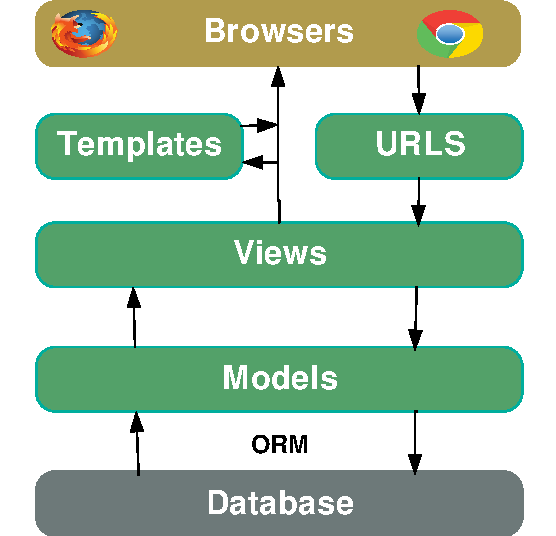
\includegraphics[scale=0.7]{fluxo_django}  %pode alterar o tamanho
						\caption[Fluxo de Informações entre Usuário e Aplicação Django]{\label{fig:fluxo_django}Fluxo de Informações entre Usuário e Aplicação Django. Adaptado de: \url{https://github.com/fga-gpp-mds/00-Disciplina/wiki/Padr\%C3\%B5es-Arquiteturais---MVC-X-Arquitetura-do-Django}}
					\end{center}		
				\end{figure}
				
				A criação de um novo projeto django é feita através do comando startproject. O comando exibido no \autoref{cod:start_project} cria um projeto chamado WebSite. O projeto criado contém alguns arquivos pré-configurados como o arquivo wsgi.py, e o settings.py. O primeiro implementa o Web Server Gateway Interface (WSGI), uma especificação que permite que a aplicação desenvolvida possa ser executada em múltiplos servidores web \cite{klaus2012}; o segundo contém configurações gerais de um site, como por exemplo, qual será o banco de dados utilizado, caminho dos arquivos estáticos, etc.
								
				\begin{listing}[!htb]
					\begin{minted}[bgcolor=bg,breaklines=true,tabsize=2, baselinestretch=1,fontsize=\footnotesize]{bash}
					# navegue até o diretóio destino da aplicação
					$ django-admin startproject WebSite
					\end{minted}
					\caption{Função que interpreta comandos vindos do WebServer}
					\label{cod:start_project}
				\end{listing}
			
				O projeto é constituído de 3 aplicações: core, operation e trend. O funcionamento das mesmas será explicado a seguir:
			
			\subsection{Aplicação Core}
				É a aplicação base do sistema. Nesta aplicação são armazenadas todos os arquivos estáticos necessários, como arquivos de imagens, arquivos de estilo (css) e arquivos javascript que são utilizados pelas demais aplicações. Esta aplicação não implementa nenhum modelo de dados, pois sua função é somente servir de sustentação para outras aplicações.
				
				O core possui dois templates: base.html e home.html. O template base consiste na estrutura geral da interface, que possui uma barra de navegação, um espaço central para inserção de conteúdo e um rodapé. Este template é utilizado pelos demais, que apenas preenchem os ``espaços'' disponibilizados no template base, para assim construir uma interface completa. A estrutura do arquivo base é mostrada no \autoref{cod:base}
				
				\begin{listing}[!htb]
					\begin{minted}[bgcolor=bg,breaklines=true,tabsize=2, baselinestretch=1,fontsize=\footnotesize]{django}
					<1 - Inicialização da estrutura padrão de um arquivo html>
					<2 - Inicialização de arquivos de estilo css comuns a todos os templates>
					<3 - Espaço para arquivos de estilo adicionais>
					<4 - Código da Barra de navegação>
					<5 - Espaço Central para inserção de conteúdo por outros templates>
					<6 - Código do rodapé>
					<7 - Inicialização de arquivos javascript comuns a todos os templates>
					<8 - Espaço para inserção de arquivos javascript adicionais>
					\end{minted}
					\caption{Template Base}
					\label{cod:base}
				\end{listing}
				
				O template home.html implementa a página inicial do sistema, que é composta por duas imagens. O template home reutiliza o template base e preenche o espaço de conteúdo disponível. Não adiciona nenhum arquivo javascript ou css. O arquivo urls possui o mapeamento para apenas uma função no arquivo views, que é a chamada para a página inicial.
				
			\subsection{Aplicação Operation}
				A aplicação operation contém o maior número de funcionalidades do projeto. Nesta aplicação, são apresentadas para o usuário as informações sobre as variáveis que representam o estado do trocador de calor, bem como estão disponíveis os componentes que permitem a intervenção do usuário sobre o sistema. Ou seja, essa interface contém basicamente displays,para exibir informações, e botões para enviar comandos do usuário para o sistema.
				
				Foram criados 3 modelos de dados para essa aplicação. Como mencionado na \duvida{seçãox}, cada modelo de dados é mapeado em uma tabela no banco de dados. O modelo Display define uma estrutura de dados para exibição de dados analógicos. Através dessa definição, torna-se fácil alterações na unidade de engenharia texto de descrição, entre outros fatores. O modelo Registers, é definido como o conjunto de informações enviadas pelo Arduino, ou seja, cada linha dessa tabela define o estado do trocador de calor em um dado instante. O modelo OperationMode consiste em armazenar informações auxiliares, como por exemplo se o armazenamento histórico está habilitado ou não. O mapeamento dessas estruturas no banco de dados está resumido na \autoref{tbl7}.
				
				\begin{table}[!htb]
					\centering
					\caption{Modelos definidos no sistema}
					\label{tbl7}
					\def\arraystretch{1.3}
					\begin{tabular}{l |l | l}
						\hline
						\multicolumn{1}{c|}{\textbf{Displays}} & \multicolumn{1}{c |}{\textbf{Registers}} &
						\multicolumn{1}{c}{\textbf{OperationMode}} \\ \hline
						
						name: string & TimeStamp: DateTime & OpMode: bool \\
						UE: string  & Temp1: float & TrendStarted: bool \\ 
						description: string & Temp2: float & \\
						Tag: string  & Temp3: float &      \\
						Value: float & Temp4: float & \\
						& HotFlow: float & \\
						& ColdFlow: float & \\
						& PumpStatus: bool & \\
						& HeaterStatus: bool & \\
						& ArduinoMode: bool & \\
						& EmergencyMode: bool & \\
						& PumpSpeed: float & \\
						\hline
					\end{tabular}
				\end{table}
				
				Essa aplicação possui 5 funções definidas na view. A função main, que é acionada quando o usuário clica para entrar nessa tela. Enquanto o usuário se mantiver nessa tela, o navegador envia requisições constantes de atualização dos dados. Essa requisição de atualização chama a função refresh, que retorna para o cliente um pacote JSON com os dados mais atuais do sistema. Essa requisição é feita via AJAX, ou seja, não provoca a atualização de toda a página, apenas dos elementos que necessitam ser atualizados, o que otimiza a performance do sistema.
				
				Quando o usuário clica em algum botão (desde que esteja habilitado), é chamada a view command, que repassa o comando para o gateway; quando o usuário movimenta o slider é chamada a view analogcommand, que repassa o comando de alteração de velocidade da bomba para o gateway. Por fim, a view export\_csv, envia os dados históricos armazenados no banco para o usuário, quando solicitado.
				
				A aplicação possui apenas um template, que reutiliza a biblioteca base e preenche o espaço de conteúdo. Para que o template funcione corretamente, foi necessário utilizar alguns arquivos css e javascript extras. A lista de arquivos e sua respectiva utilidade é descrita na \autoref{tbl8}. Para que cada botão consiga enviar o respectivo comando para a view, criou-se um parâmetro que recebe um índice de comando. Os números atribuídos são os mesmos definidos na \autoref{tbl5}. A diferença é que no arquivo de template a representação do comando está em char, enquanto na tabela consta a representação do comando em decimal. Isso ocorre porque o Arduino interpreta o comando, que foi enviado na forma de string, através da representação decimal. A relação entre um caractere e sua representação numérica pode ser consultada na tabela ASCII\footnote{\url{https://en.wikipedia.org/wiki/ASCII}}.
				
				\begin{table}[!htb]
					\centering
					\caption{Arquivos extras utilizados pela aplicação}
					\label{tbl8}
					\def\arraystretch{1.3}
					\begin{tabular}{l p{11cm}}
						\hline
						\multicolumn{1}{c}{\textbf{Arquivo}} & \multicolumn{1}{c }{\textbf{Função}} \\ \hline
						bootstrap-slider.css & Biblioteca mantida por \textcite{rohit2017}, \\
						bootstrap-slider.js & que implementa o objeto slider da aplicação \\ \hline
						raphael-2.1.4.js & Biblioteca mantida por
						\textcite{bojan2016}, que implementa \\
						justgage.js & o objeto gauge (barra de nível circular) da aplicação \\ \hline
						bootstrap-confirmation.js & Biblioteca mantida por \textcite{damien2017} que implementa a confirmação após clique de botões \\ \hline
						operation.js & Arquivo que executa a solicitação cíclica de dados para o servidor, bem como interpreta o retorno e atualiza a página para o usuário. Também monitora os eventos dos botões, e quando algum evento ocorre, envia os comandos para o servidor. \\		
						
						\hline
					\end{tabular}
				\end{table}
				
				
				
				
				
				
					
				
				